\documentclass[twoside]{book}

% Packages required by doxygen
\usepackage{fixltx2e}
\usepackage{calc}
\usepackage{doxygen}
\usepackage[export]{adjustbox} % also loads graphicx
\usepackage{graphicx}
\usepackage[utf8]{inputenc}
\usepackage{makeidx}
\usepackage{multicol}
\usepackage{multirow}
\PassOptionsToPackage{warn}{textcomp}
\usepackage{textcomp}
\usepackage[nointegrals]{wasysym}
\usepackage[table]{xcolor}

% Font selection
\usepackage[T1]{fontenc}
\usepackage[scaled=.90]{helvet}
\usepackage{courier}
\usepackage{amssymb}
\usepackage{sectsty}
\renewcommand{\familydefault}{\sfdefault}
\allsectionsfont{%
  \fontseries{bc}\selectfont%
  \color{darkgray}%
}
\renewcommand{\DoxyLabelFont}{%
  \fontseries{bc}\selectfont%
  \color{darkgray}%
}
\newcommand{\+}{\discretionary{\mbox{\scriptsize$\hookleftarrow$}}{}{}}

% Page & text layout
\usepackage{geometry}
\geometry{%
  a4paper,%
  top=2.5cm,%
  bottom=2.5cm,%
  left=2.5cm,%
  right=2.5cm%
}
\tolerance=750
\hfuzz=15pt
\hbadness=750
\setlength{\emergencystretch}{15pt}
\setlength{\parindent}{0cm}
\setlength{\parskip}{3ex plus 2ex minus 2ex}
\makeatletter
\renewcommand{\paragraph}{%
  \@startsection{paragraph}{4}{0ex}{-1.0ex}{1.0ex}{%
    \normalfont\normalsize\bfseries\SS@parafont%
  }%
}
\renewcommand{\subparagraph}{%
  \@startsection{subparagraph}{5}{0ex}{-1.0ex}{1.0ex}{%
    \normalfont\normalsize\bfseries\SS@subparafont%
  }%
}
\makeatother

% Headers & footers
\usepackage{fancyhdr}
\pagestyle{fancyplain}
\fancyhead[LE]{\fancyplain{}{\bfseries\thepage}}
\fancyhead[CE]{\fancyplain{}{}}
\fancyhead[RE]{\fancyplain{}{\bfseries\leftmark}}
\fancyhead[LO]{\fancyplain{}{\bfseries\rightmark}}
\fancyhead[CO]{\fancyplain{}{}}
\fancyhead[RO]{\fancyplain{}{\bfseries\thepage}}
\fancyfoot[LE]{\fancyplain{}{}}
\fancyfoot[CE]{\fancyplain{}{}}
\fancyfoot[RE]{\fancyplain{}{\bfseries\scriptsize Generated by Doxygen }}
\fancyfoot[LO]{\fancyplain{}{\bfseries\scriptsize Generated by Doxygen }}
\fancyfoot[CO]{\fancyplain{}{}}
\fancyfoot[RO]{\fancyplain{}{}}
\renewcommand{\footrulewidth}{0.4pt}
\renewcommand{\chaptermark}[1]{%
  \markboth{#1}{}%
}
\renewcommand{\sectionmark}[1]{%
  \markright{\thesection\ #1}%
}

% Indices & bibliography
\usepackage{natbib}
\usepackage[titles]{tocloft}
\setcounter{tocdepth}{3}
\setcounter{secnumdepth}{5}
\makeindex

% Hyperlinks (required, but should be loaded last)
\usepackage{ifpdf}
\ifpdf
  \usepackage[pdftex,pagebackref=true]{hyperref}
\else
  \usepackage[ps2pdf,pagebackref=true]{hyperref}
\fi
\hypersetup{%
  colorlinks=true,%
  linkcolor=blue,%
  citecolor=blue,%
  unicode%
}

% Custom commands
\newcommand{\clearemptydoublepage}{%
  \newpage{\pagestyle{empty}\cleardoublepage}%
}

\usepackage{caption}
\captionsetup{labelsep=space,justification=centering,font={bf},singlelinecheck=off,skip=4pt,position=top}

%===== C O N T E N T S =====

\begin{document}

% Titlepage & ToC
\hypersetup{pageanchor=false,
             bookmarksnumbered=true,
             pdfencoding=unicode
            }
\pagenumbering{alph}
\begin{titlepage}
\vspace*{7cm}
\begin{center}%
{\Large My Project }\\
\vspace*{1cm}
{\large Generated by Doxygen 1.8.13}\\
\end{center}
\end{titlepage}
\clearemptydoublepage
\pagenumbering{roman}
\tableofcontents
\clearemptydoublepage
\pagenumbering{arabic}
\hypersetup{pageanchor=true}

%--- Begin generated contents ---
\chapter{Hierarchical Index}
\section{Class Hierarchy}
This inheritance list is sorted roughly, but not completely, alphabetically\+:\begin{DoxyCompactList}
\item \contentsline{section}{Container}{\pageref{classContainer}}{}
\begin{DoxyCompactList}
\item \contentsline{section}{Crafting\+Table}{\pageref{classCraftingTable}}{}
\end{DoxyCompactList}
\item \contentsline{section}{Exception}{\pageref{classException}}{}
\begin{DoxyCompactList}
\item \contentsline{section}{Different\+Item\+Target\+Exception}{\pageref{classDifferentItemTargetException}}{}
\item \contentsline{section}{Empty\+Source\+Exception}{\pageref{classEmptySourceException}}{}
\item \contentsline{section}{Failed\+Craft\+Exception}{\pageref{classFailedCraftException}}{}
\item \contentsline{section}{Full\+Inventory\+Exception}{\pageref{classFullInventoryException}}{}
\item \contentsline{section}{Invalid\+Quantity\+Exception}{\pageref{classInvalidQuantityException}}{}
\item \contentsline{section}{Not\+Enough\+Item\+Exception}{\pageref{classNotEnoughItemException}}{}
\item \contentsline{section}{Out\+Of\+Range\+Exception}{\pageref{classOutOfRangeException}}{}
\end{DoxyCompactList}
\item \contentsline{section}{Item}{\pageref{classItem}}{}
\begin{DoxyCompactList}
\item \contentsline{section}{Non\+Tool}{\pageref{classNonTool}}{}
\item \contentsline{section}{Tool}{\pageref{classTool}}{}
\end{DoxyCompactList}
\item \contentsline{section}{Recipe}{\pageref{classRecipe}}{}
\end{DoxyCompactList}

\chapter{Class Index}
\section{Class List}
Here are the classes, structs, unions and interfaces with brief descriptions\+:\begin{DoxyCompactList}
\item\contentsline{section}{\hyperlink{classContainer}{Container} }{\pageref{classContainer}}{}
\item\contentsline{section}{\hyperlink{classCraftingTable}{Crafting\+Table} }{\pageref{classCraftingTable}}{}
\item\contentsline{section}{\hyperlink{classDifferentItemTargetException}{Different\+Item\+Target\+Exception} }{\pageref{classDifferentItemTargetException}}{}
\item\contentsline{section}{\hyperlink{classEmptySourceException}{Empty\+Source\+Exception} }{\pageref{classEmptySourceException}}{}
\item\contentsline{section}{\hyperlink{classException}{Exception} }{\pageref{classException}}{}
\item\contentsline{section}{\hyperlink{classFailedCraftException}{Failed\+Craft\+Exception} }{\pageref{classFailedCraftException}}{}
\item\contentsline{section}{\hyperlink{classFullInventoryException}{Full\+Inventory\+Exception} }{\pageref{classFullInventoryException}}{}
\item\contentsline{section}{\hyperlink{classInvalidQuantityException}{Invalid\+Quantity\+Exception} }{\pageref{classInvalidQuantityException}}{}
\item\contentsline{section}{\hyperlink{classItem}{Item} }{\pageref{classItem}}{}
\item\contentsline{section}{\hyperlink{classNonTool}{Non\+Tool} }{\pageref{classNonTool}}{}
\item\contentsline{section}{\hyperlink{classNotEnoughItemException}{Not\+Enough\+Item\+Exception} }{\pageref{classNotEnoughItemException}}{}
\item\contentsline{section}{\hyperlink{classOutOfRangeException}{Out\+Of\+Range\+Exception} }{\pageref{classOutOfRangeException}}{}
\item\contentsline{section}{\hyperlink{classRecipe}{Recipe} }{\pageref{classRecipe}}{}
\item\contentsline{section}{\hyperlink{classTool}{Tool} }{\pageref{classTool}}{}
\end{DoxyCompactList}

\chapter{Class Documentation}
\hypertarget{classContainer}{}\section{Container Class Reference}
\label{classContainer}\index{Container@{Container}}


Inheritance diagram for Container\+:
\nopagebreak
\begin{figure}[H]
\begin{center}
\leavevmode
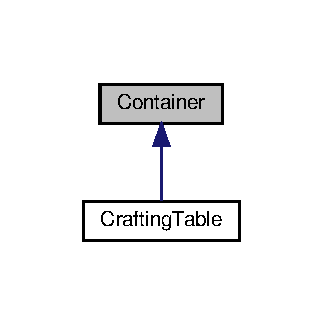
\includegraphics[width=155pt]{classContainer__inherit__graph}
\end{center}
\end{figure}


Collaboration diagram for Container\+:
\nopagebreak
\begin{figure}[H]
\begin{center}
\leavevmode
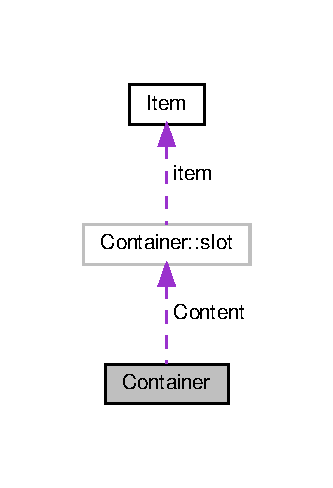
\includegraphics[width=160pt]{classContainer__coll__graph}
\end{center}
\end{figure}
\subsection*{Public Member Functions}
\begin{DoxyCompactItemize}
\item 
\mbox{\Hypertarget{classContainer_a3cffc4a781ade773f436ac8d7e93ea1f}\label{classContainer_a3cffc4a781ade773f436ac8d7e93ea1f}} 
{\bfseries Container} (int size)
\item 
\mbox{\Hypertarget{classContainer_a2380b9e12e08f17ad1d97607b87e16be}\label{classContainer_a2380b9e12e08f17ad1d97607b87e16be}} 
Slot {\bfseries get\+Item} (int index)
\item 
\mbox{\Hypertarget{classContainer_a8f17aec1ba74eb14336624b2141c4ba3}\label{classContainer_a8f17aec1ba74eb14336624b2141c4ba3}} 
int {\bfseries get\+Size} ()
\item 
\mbox{\Hypertarget{classContainer_a3abf81a8cce653a85ce6073c511d79a2}\label{classContainer_a3abf81a8cce653a85ce6073c511d79a2}} 
void {\bfseries insert} (int n, \hyperlink{classItem}{Item} \&itemX)
\item 
\mbox{\Hypertarget{classContainer_a34218839d4c35dd9ccc101d4eb71f7aa}\label{classContainer_a34218839d4c35dd9ccc101d4eb71f7aa}} 
void {\bfseries insert} (\hyperlink{classItem}{Item} \&itemX, int durability)
\item 
\mbox{\Hypertarget{classContainer_a328733f18186b3fcca0c787745193c24}\label{classContainer_a328733f18186b3fcca0c787745193c24}} 
void {\bfseries insert} (int n, \hyperlink{classItem}{Item} \&itemX, int index)
\item 
\mbox{\Hypertarget{classContainer_adccb8b9e861e6710c4d08d348245662f}\label{classContainer_adccb8b9e861e6710c4d08d348245662f}} 
void {\bfseries discard} (int index, int n)
\item 
\mbox{\Hypertarget{classContainer_a84ae6595aef25e44a4786b0d2bd2c172}\label{classContainer_a84ae6595aef25e44a4786b0d2bd2c172}} 
void {\bfseries display} ()
\end{DoxyCompactItemize}
\subsection*{Static Public Member Functions}
\begin{DoxyCompactItemize}
\item 
\mbox{\Hypertarget{classContainer_a1b76b03655880a4e7abb5980edcf4d65}\label{classContainer_a1b76b03655880a4e7abb5980edcf4d65}} 
static void {\bfseries move} (\hyperlink{classContainer}{Container} \&src, int src\+Idx, \hyperlink{classContainer}{Container} \&dst, int dst\+Idx)
\item 
\mbox{\Hypertarget{classContainer_aeed5f1e2c7df9a0feb5dad9d28e6fcd0}\label{classContainer_aeed5f1e2c7df9a0feb5dad9d28e6fcd0}} 
static void {\bfseries move} (\hyperlink{classContainer}{Container} \&src, int src\+Idx, \hyperlink{classContainer}{Container} \&dst, int dst\+Idx, int n)
\item 
\mbox{\Hypertarget{classContainer_a37bc648372a93c699ea716f5ca879dd9}\label{classContainer_a37bc648372a93c699ea716f5ca879dd9}} 
static void {\bfseries swap} (\hyperlink{classContainer}{Container} \&src, int src\+Idx, \hyperlink{classContainer}{Container} \&dst, int dst\+Idx)
\end{DoxyCompactItemize}
\subsection*{Protected Attributes}
\begin{DoxyCompactItemize}
\item 
\mbox{\Hypertarget{classContainer_af0f10443591de588f0a85b62f73ffc82}\label{classContainer_af0f10443591de588f0a85b62f73ffc82}} 
int {\bfseries size}
\item 
\mbox{\Hypertarget{classContainer_ab44f803cb2815683353619aaed2e70ac}\label{classContainer_ab44f803cb2815683353619aaed2e70ac}} 
Slot $\ast$ {\bfseries Content}
\end{DoxyCompactItemize}


The documentation for this class was generated from the following file\+:\begin{DoxyCompactItemize}
\item 
Container.\+hpp\end{DoxyCompactItemize}

\hypertarget{classCraftingTable}{}\section{Crafting\+Table Class Reference}
\label{classCraftingTable}\index{Crafting\+Table@{Crafting\+Table}}


Inheritance diagram for Crafting\+Table\+:
\nopagebreak
\begin{figure}[H]
\begin{center}
\leavevmode
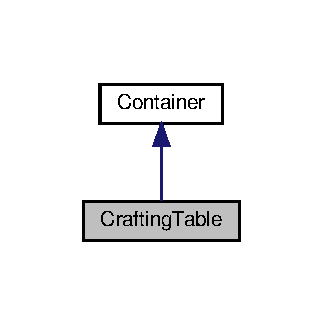
\includegraphics[width=155pt]{classCraftingTable__inherit__graph}
\end{center}
\end{figure}


Collaboration diagram for Crafting\+Table\+:
\nopagebreak
\begin{figure}[H]
\begin{center}
\leavevmode
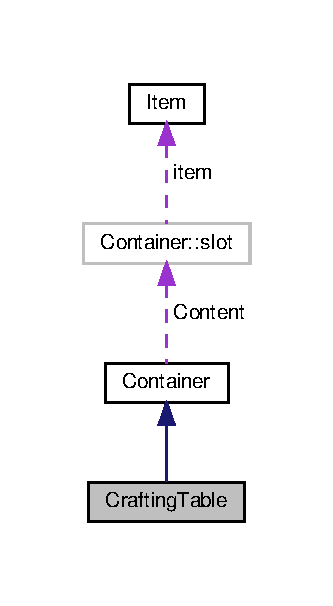
\includegraphics[width=160pt]{classCraftingTable__coll__graph}
\end{center}
\end{figure}
\subsection*{Public Member Functions}
\begin{DoxyCompactItemize}
\item 
\mbox{\Hypertarget{classCraftingTable_a36f5d86a261109862bfa7694eda5b184}\label{classCraftingTable_a36f5d86a261109862bfa7694eda5b184}} 
string {\bfseries get\+Name} (int n)
\item 
\mbox{\Hypertarget{classCraftingTable_a9fdc40661df46962243650b87707efc9}\label{classCraftingTable_a9fdc40661df46962243650b87707efc9}} 
string {\bfseries get\+Type} (int n)
\item 
\mbox{\Hypertarget{classCraftingTable_aa6c8c5a429043f061028ed71d355d135}\label{classCraftingTable_aa6c8c5a429043f061028ed71d355d135}} 
bool {\bfseries is\+Empty} ()
\item 
\mbox{\Hypertarget{classCraftingTable_aa130ad45ab41cae52174f0acabfcb2e3}\label{classCraftingTable_aa130ad45ab41cae52174f0acabfcb2e3}} 
bool {\bfseries is\+Tool} ()
\item 
\mbox{\Hypertarget{classCraftingTable_ab96e041f3c9789c85cd5aca26dd0ae51}\label{classCraftingTable_ab96e041f3c9789c85cd5aca26dd0ae51}} 
bool {\bfseries is\+Non\+Tool} ()
\item 
\mbox{\Hypertarget{classCraftingTable_a29f94729f67f3035649b3ae78e508997}\label{classCraftingTable_a29f94729f67f3035649b3ae78e508997}} 
bool {\bfseries check} (string $\ast$)
\item 
\mbox{\Hypertarget{classCraftingTable_af04bf32ed068072a41abb68d11b13672}\label{classCraftingTable_af04bf32ed068072a41abb68d11b13672}} 
bool {\bfseries check\+Mirror} (string $\ast$)
\item 
\mbox{\Hypertarget{classCraftingTable_a1e644f6269af59ae8315a2ca7fd651c0}\label{classCraftingTable_a1e644f6269af59ae8315a2ca7fd651c0}} 
bool {\bfseries check\+Sub} (string $\ast$, int, int)
\item 
\mbox{\Hypertarget{classCraftingTable_ab59eff677f8e20f5914f7308e4dfc28c}\label{classCraftingTable_ab59eff677f8e20f5914f7308e4dfc28c}} 
void {\bfseries craft} (\hyperlink{classContainer}{Container} \&)
\end{DoxyCompactItemize}
\subsection*{Additional Inherited Members}


The documentation for this class was generated from the following file\+:\begin{DoxyCompactItemize}
\item 
Crafting\+Table.\+hpp\end{DoxyCompactItemize}

\hypertarget{classDifferentItemTargetException}{}\section{Different\+Item\+Target\+Exception Class Reference}
\label{classDifferentItemTargetException}\index{Different\+Item\+Target\+Exception@{Different\+Item\+Target\+Exception}}


Inheritance diagram for Different\+Item\+Target\+Exception\+:
\nopagebreak
\begin{figure}[H]
\begin{center}
\leavevmode
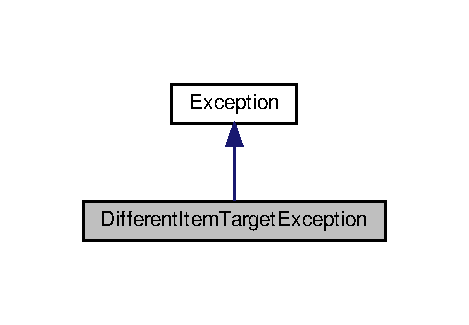
\includegraphics[width=225pt]{classDifferentItemTargetException__inherit__graph}
\end{center}
\end{figure}


Collaboration diagram for Different\+Item\+Target\+Exception\+:
\nopagebreak
\begin{figure}[H]
\begin{center}
\leavevmode
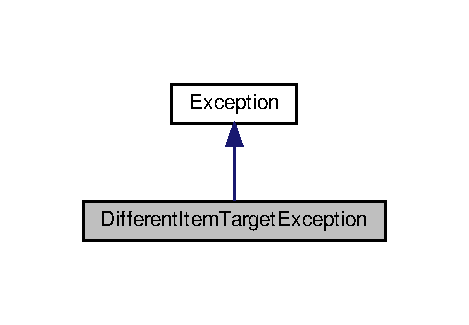
\includegraphics[width=225pt]{classDifferentItemTargetException__coll__graph}
\end{center}
\end{figure}
\subsection*{Public Member Functions}
\begin{DoxyCompactItemize}
\item 
\mbox{\Hypertarget{classDifferentItemTargetException_a3566195af75854aef6d1b7f56b9ba15d}\label{classDifferentItemTargetException_a3566195af75854aef6d1b7f56b9ba15d}} 
string {\bfseries what} ()
\end{DoxyCompactItemize}


The documentation for this class was generated from the following file\+:\begin{DoxyCompactItemize}
\item 
Exception.\+hpp\end{DoxyCompactItemize}

\hypertarget{classEmptySourceException}{}\section{Empty\+Source\+Exception Class Reference}
\label{classEmptySourceException}\index{Empty\+Source\+Exception@{Empty\+Source\+Exception}}


Inheritance diagram for Empty\+Source\+Exception\+:
\nopagebreak
\begin{figure}[H]
\begin{center}
\leavevmode
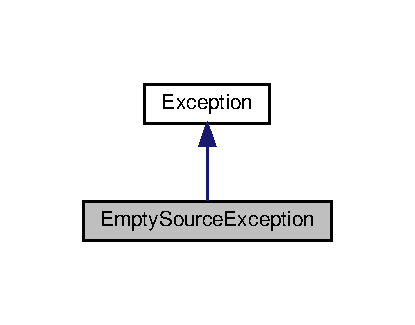
\includegraphics[width=199pt]{classEmptySourceException__inherit__graph}
\end{center}
\end{figure}


Collaboration diagram for Empty\+Source\+Exception\+:
\nopagebreak
\begin{figure}[H]
\begin{center}
\leavevmode
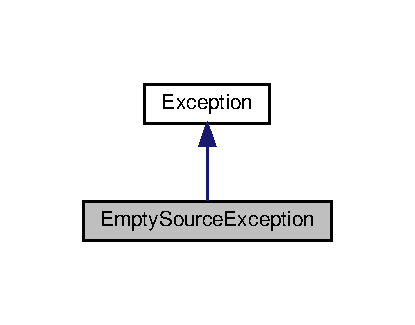
\includegraphics[width=199pt]{classEmptySourceException__coll__graph}
\end{center}
\end{figure}
\subsection*{Public Member Functions}
\begin{DoxyCompactItemize}
\item 
\mbox{\Hypertarget{classEmptySourceException_a0d97e2edacbd6dda86b098ac79fffe78}\label{classEmptySourceException_a0d97e2edacbd6dda86b098ac79fffe78}} 
string {\bfseries what} ()
\end{DoxyCompactItemize}


The documentation for this class was generated from the following file\+:\begin{DoxyCompactItemize}
\item 
Exception.\+hpp\end{DoxyCompactItemize}

\hypertarget{classException}{}\section{Exception Class Reference}
\label{classException}\index{Exception@{Exception}}


Inheritance diagram for Exception\+:
\nopagebreak
\begin{figure}[H]
\begin{center}
\leavevmode
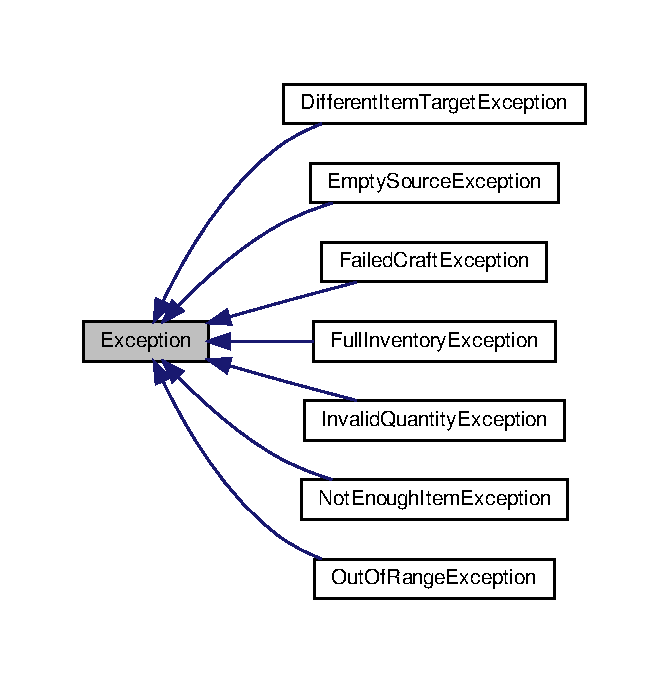
\includegraphics[width=321pt]{classException__inherit__graph}
\end{center}
\end{figure}
\subsection*{Public Member Functions}
\begin{DoxyCompactItemize}
\item 
\mbox{\Hypertarget{classException_ab7dc9e19c7ebf82d3e345ffeb4778138}\label{classException_ab7dc9e19c7ebf82d3e345ffeb4778138}} 
virtual string {\bfseries what} ()=0
\end{DoxyCompactItemize}


The documentation for this class was generated from the following file\+:\begin{DoxyCompactItemize}
\item 
Exception.\+hpp\end{DoxyCompactItemize}

\hypertarget{classFailedCraftException}{}\section{Failed\+Craft\+Exception Class Reference}
\label{classFailedCraftException}\index{Failed\+Craft\+Exception@{Failed\+Craft\+Exception}}


Inheritance diagram for Failed\+Craft\+Exception\+:
\nopagebreak
\begin{figure}[H]
\begin{center}
\leavevmode
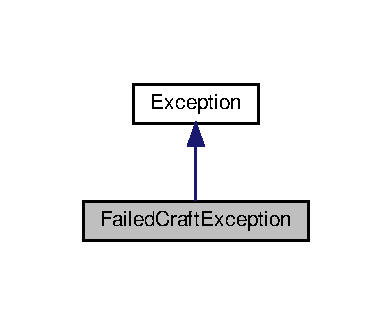
\includegraphics[width=188pt]{classFailedCraftException__inherit__graph}
\end{center}
\end{figure}


Collaboration diagram for Failed\+Craft\+Exception\+:
\nopagebreak
\begin{figure}[H]
\begin{center}
\leavevmode
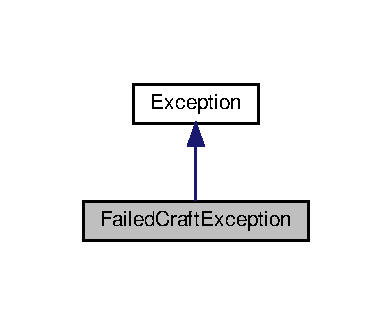
\includegraphics[width=188pt]{classFailedCraftException__coll__graph}
\end{center}
\end{figure}
\subsection*{Public Member Functions}
\begin{DoxyCompactItemize}
\item 
\mbox{\Hypertarget{classFailedCraftException_a520c879bea5c8800089629219861cc63}\label{classFailedCraftException_a520c879bea5c8800089629219861cc63}} 
string {\bfseries what} ()
\end{DoxyCompactItemize}


The documentation for this class was generated from the following file\+:\begin{DoxyCompactItemize}
\item 
Exception.\+hpp\end{DoxyCompactItemize}

\hypertarget{classFullInventoryException}{}\section{Full\+Inventory\+Exception Class Reference}
\label{classFullInventoryException}\index{Full\+Inventory\+Exception@{Full\+Inventory\+Exception}}


Inheritance diagram for Full\+Inventory\+Exception\+:
\nopagebreak
\begin{figure}[H]
\begin{center}
\leavevmode
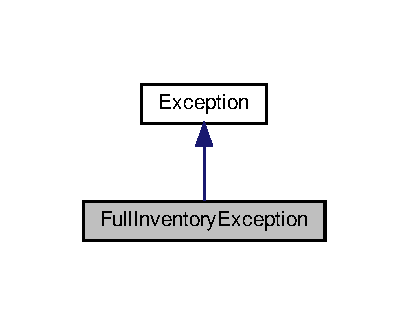
\includegraphics[width=196pt]{classFullInventoryException__inherit__graph}
\end{center}
\end{figure}


Collaboration diagram for Full\+Inventory\+Exception\+:
\nopagebreak
\begin{figure}[H]
\begin{center}
\leavevmode
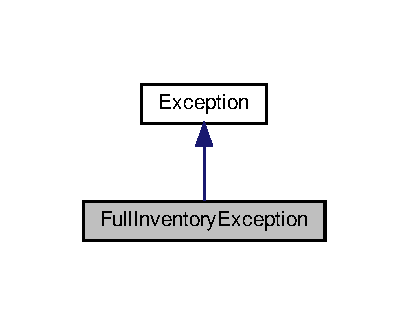
\includegraphics[width=196pt]{classFullInventoryException__coll__graph}
\end{center}
\end{figure}
\subsection*{Public Member Functions}
\begin{DoxyCompactItemize}
\item 
\mbox{\Hypertarget{classFullInventoryException_ac3bba389ec79cd23c88c22084f1c4548}\label{classFullInventoryException_ac3bba389ec79cd23c88c22084f1c4548}} 
string {\bfseries what} ()
\end{DoxyCompactItemize}


The documentation for this class was generated from the following file\+:\begin{DoxyCompactItemize}
\item 
Exception.\+hpp\end{DoxyCompactItemize}

\hypertarget{classInvalidQuantityException}{}\section{Invalid\+Quantity\+Exception Class Reference}
\label{classInvalidQuantityException}\index{Invalid\+Quantity\+Exception@{Invalid\+Quantity\+Exception}}


Inheritance diagram for Invalid\+Quantity\+Exception\+:
\nopagebreak
\begin{figure}[H]
\begin{center}
\leavevmode
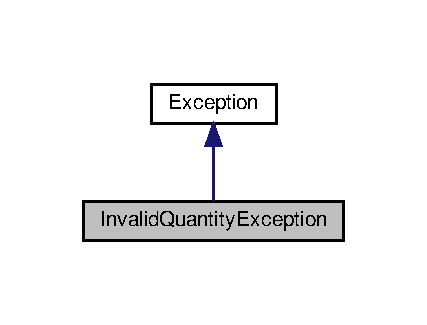
\includegraphics[width=205pt]{classInvalidQuantityException__inherit__graph}
\end{center}
\end{figure}


Collaboration diagram for Invalid\+Quantity\+Exception\+:
\nopagebreak
\begin{figure}[H]
\begin{center}
\leavevmode
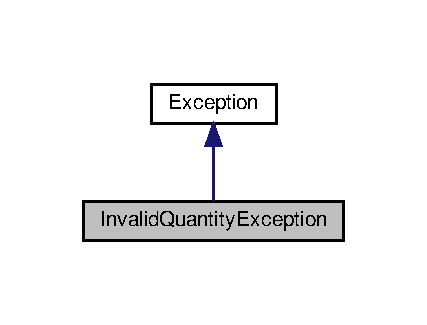
\includegraphics[width=205pt]{classInvalidQuantityException__coll__graph}
\end{center}
\end{figure}
\subsection*{Public Member Functions}
\begin{DoxyCompactItemize}
\item 
\mbox{\Hypertarget{classInvalidQuantityException_a1e880d8b67ea560423b24aa2113bda55}\label{classInvalidQuantityException_a1e880d8b67ea560423b24aa2113bda55}} 
string {\bfseries what} ()
\end{DoxyCompactItemize}


The documentation for this class was generated from the following file\+:\begin{DoxyCompactItemize}
\item 
Exception.\+hpp\end{DoxyCompactItemize}

\hypertarget{classItem}{}\section{Item Class Reference}
\label{classItem}\index{Item@{Item}}


Inheritance diagram for Item\+:
\nopagebreak
\begin{figure}[H]
\begin{center}
\leavevmode
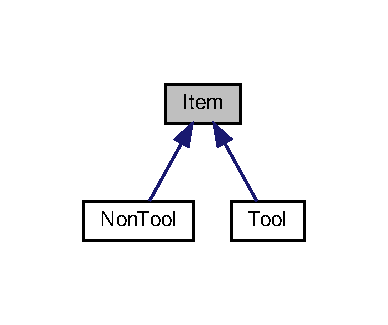
\includegraphics[width=186pt]{classItem__inherit__graph}
\end{center}
\end{figure}
\subsection*{Public Member Functions}
\begin{DoxyCompactItemize}
\item 
\mbox{\Hypertarget{classItem_ac909c537a0cc1e16cc8a20b5a31e8ae7}\label{classItem_ac909c537a0cc1e16cc8a20b5a31e8ae7}} 
{\bfseries Item} (int id, string name, Item\+Type type)
\item 
\mbox{\Hypertarget{classItem_a73c0ea2b51684e195f886c269b841434}\label{classItem_a73c0ea2b51684e195f886c269b841434}} 
int {\bfseries get\+ID} ()
\item 
\mbox{\Hypertarget{classItem_a63d7f2148b699e539aae354b01559811}\label{classItem_a63d7f2148b699e539aae354b01559811}} 
string {\bfseries get\+Name} ()
\item 
\mbox{\Hypertarget{classItem_a4a649a87af64ef21c82fbff3c203cb41}\label{classItem_a4a649a87af64ef21c82fbff3c203cb41}} 
Item\+Type {\bfseries get\+Type} ()
\item 
\mbox{\Hypertarget{classItem_a6b049623f6561d8da1cd6739f7b4f87c}\label{classItem_a6b049623f6561d8da1cd6739f7b4f87c}} 
string {\bfseries get\+Type\+To\+String} ()
\item 
\mbox{\Hypertarget{classItem_a145525994415170e36651e7ef1dee8ef}\label{classItem_a145525994415170e36651e7ef1dee8ef}} 
virtual string {\bfseries output} (int)=0
\end{DoxyCompactItemize}
\subsection*{Protected Attributes}
\begin{DoxyCompactItemize}
\item 
\mbox{\Hypertarget{classItem_a3a58b8b450282d765d8ab445b7e6a4e3}\label{classItem_a3a58b8b450282d765d8ab445b7e6a4e3}} 
Item\+Type {\bfseries type}
\item 
\mbox{\Hypertarget{classItem_ae901ac3ab2273113f746340a7db4e388}\label{classItem_ae901ac3ab2273113f746340a7db4e388}} 
int {\bfseries id}
\item 
\mbox{\Hypertarget{classItem_a406cde7962a6b42a66b4a53c9a26db2c}\label{classItem_a406cde7962a6b42a66b4a53c9a26db2c}} 
string {\bfseries name}
\end{DoxyCompactItemize}


The documentation for this class was generated from the following file\+:\begin{DoxyCompactItemize}
\item 
Item.\+hpp\end{DoxyCompactItemize}

\hypertarget{classNonTool}{}\section{Non\+Tool Class Reference}
\label{classNonTool}\index{Non\+Tool@{Non\+Tool}}


Inheritance diagram for Non\+Tool\+:
\nopagebreak
\begin{figure}[H]
\begin{center}
\leavevmode
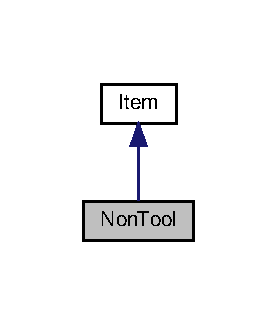
\includegraphics[width=133pt]{classNonTool__inherit__graph}
\end{center}
\end{figure}


Collaboration diagram for Non\+Tool\+:
\nopagebreak
\begin{figure}[H]
\begin{center}
\leavevmode
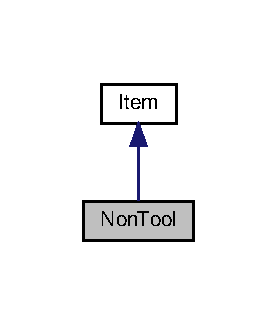
\includegraphics[width=133pt]{classNonTool__coll__graph}
\end{center}
\end{figure}
\subsection*{Public Member Functions}
\begin{DoxyCompactItemize}
\item 
\mbox{\Hypertarget{classNonTool_a401a2fdd6bb0a5f08fe1bb624d24cac4}\label{classNonTool_a401a2fdd6bb0a5f08fe1bb624d24cac4}} 
{\bfseries Non\+Tool} (int id, std\+::string name, Item\+Type type)
\item 
\mbox{\Hypertarget{classNonTool_a041faeae0c0bdb98ba41079a1773b6f2}\label{classNonTool_a041faeae0c0bdb98ba41079a1773b6f2}} 
\hyperlink{classNonTool}{Non\+Tool} {\bfseries operator=} (const \hyperlink{classNonTool}{Non\+Tool} \&other)
\item 
\mbox{\Hypertarget{classNonTool_ac4dcee4d5d2f0e8c03aa80103baacc3f}\label{classNonTool_ac4dcee4d5d2f0e8c03aa80103baacc3f}} 
string {\bfseries output} (int qty) override
\end{DoxyCompactItemize}
\subsection*{Additional Inherited Members}


The documentation for this class was generated from the following file\+:\begin{DoxyCompactItemize}
\item 
Non\+Tool.\+hpp\end{DoxyCompactItemize}

\hypertarget{classNotEnoughItemException}{}\section{Not\+Enough\+Item\+Exception Class Reference}
\label{classNotEnoughItemException}\index{Not\+Enough\+Item\+Exception@{Not\+Enough\+Item\+Exception}}


Inheritance diagram for Not\+Enough\+Item\+Exception\+:
\nopagebreak
\begin{figure}[H]
\begin{center}
\leavevmode
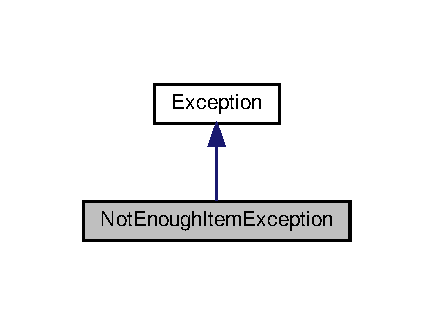
\includegraphics[width=208pt]{classNotEnoughItemException__inherit__graph}
\end{center}
\end{figure}


Collaboration diagram for Not\+Enough\+Item\+Exception\+:
\nopagebreak
\begin{figure}[H]
\begin{center}
\leavevmode
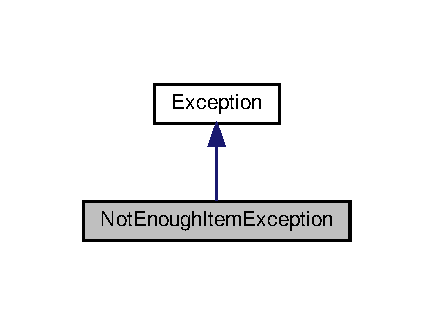
\includegraphics[width=208pt]{classNotEnoughItemException__coll__graph}
\end{center}
\end{figure}
\subsection*{Public Member Functions}
\begin{DoxyCompactItemize}
\item 
\mbox{\Hypertarget{classNotEnoughItemException_a750953eb87c1c4c2323c082fddb2b038}\label{classNotEnoughItemException_a750953eb87c1c4c2323c082fddb2b038}} 
string {\bfseries what} ()
\end{DoxyCompactItemize}


The documentation for this class was generated from the following file\+:\begin{DoxyCompactItemize}
\item 
Exception.\+hpp\end{DoxyCompactItemize}

\hypertarget{classOutOfRangeException}{}\section{Out\+Of\+Range\+Exception Class Reference}
\label{classOutOfRangeException}\index{Out\+Of\+Range\+Exception@{Out\+Of\+Range\+Exception}}


Inheritance diagram for Out\+Of\+Range\+Exception\+:
\nopagebreak
\begin{figure}[H]
\begin{center}
\leavevmode
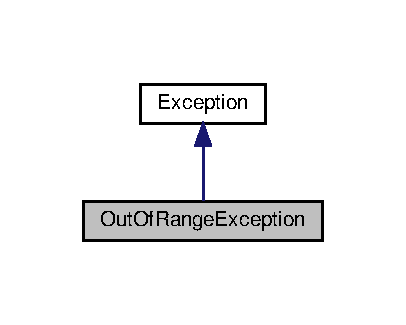
\includegraphics[width=195pt]{classOutOfRangeException__inherit__graph}
\end{center}
\end{figure}


Collaboration diagram for Out\+Of\+Range\+Exception\+:
\nopagebreak
\begin{figure}[H]
\begin{center}
\leavevmode
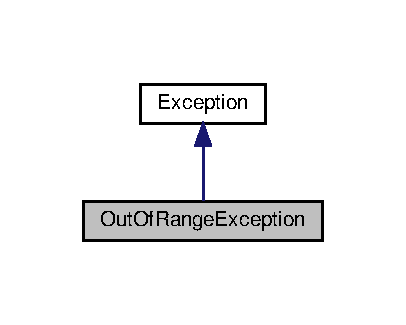
\includegraphics[width=195pt]{classOutOfRangeException__coll__graph}
\end{center}
\end{figure}
\subsection*{Public Member Functions}
\begin{DoxyCompactItemize}
\item 
\mbox{\Hypertarget{classOutOfRangeException_a1154ecb3ad64bd2f044d834ccc8d63ea}\label{classOutOfRangeException_a1154ecb3ad64bd2f044d834ccc8d63ea}} 
string {\bfseries what} ()
\end{DoxyCompactItemize}


The documentation for this class was generated from the following file\+:\begin{DoxyCompactItemize}
\item 
Exception.\+hpp\end{DoxyCompactItemize}

\hypertarget{classRecipe}{}\section{Recipe Class Reference}
\label{classRecipe}\index{Recipe@{Recipe}}
\subsection*{Public Member Functions}
\begin{DoxyCompactItemize}
\item 
\mbox{\Hypertarget{classRecipe_aaf4b2e6b0282fa19c6381947099d25a7}\label{classRecipe_aaf4b2e6b0282fa19c6381947099d25a7}} 
{\bfseries Recipe} (int, int)
\item 
\mbox{\Hypertarget{classRecipe_a3e6b4889244567c3c474e3ee01d26975}\label{classRecipe_a3e6b4889244567c3c474e3ee01d26975}} 
void {\bfseries set\+Row} (int)
\item 
\mbox{\Hypertarget{classRecipe_a4c01c8c3c014f40fae53936b03dbb7e6}\label{classRecipe_a4c01c8c3c014f40fae53936b03dbb7e6}} 
int {\bfseries get\+Row} () const
\item 
\mbox{\Hypertarget{classRecipe_aef70a9a1d8e39b5f09c9287c1fc5abb9}\label{classRecipe_aef70a9a1d8e39b5f09c9287c1fc5abb9}} 
void {\bfseries set\+Column} (int)
\item 
\mbox{\Hypertarget{classRecipe_a2c965c18e26d9cb04c065b049699865f}\label{classRecipe_a2c965c18e26d9cb04c065b049699865f}} 
int {\bfseries get\+Column} () const
\item 
\mbox{\Hypertarget{classRecipe_ad4653f2df220db08d754cc84ee987a3f}\label{classRecipe_ad4653f2df220db08d754cc84ee987a3f}} 
void {\bfseries set\+Blueprint} (int, string)
\item 
\mbox{\Hypertarget{classRecipe_a39aef1118df41ff15aa25d2fb39ab863}\label{classRecipe_a39aef1118df41ff15aa25d2fb39ab863}} 
string $\ast$ {\bfseries get\+Blueprint} ()
\item 
\mbox{\Hypertarget{classRecipe_a192cd352444d58e6554a686539d364dd}\label{classRecipe_a192cd352444d58e6554a686539d364dd}} 
string {\bfseries operator\mbox{[}$\,$\mbox{]}} (int)
\item 
\mbox{\Hypertarget{classRecipe_a343c41ba9e90331c361d4588113976d6}\label{classRecipe_a343c41ba9e90331c361d4588113976d6}} 
void {\bfseries set\+Item\+Name} (string)
\item 
\mbox{\Hypertarget{classRecipe_a6e40b01a85250263b2f971581b99175d}\label{classRecipe_a6e40b01a85250263b2f971581b99175d}} 
string {\bfseries get\+Item\+Name} () const
\item 
\mbox{\Hypertarget{classRecipe_af633e1415ad1b7a2d1dca9078632d1eb}\label{classRecipe_af633e1415ad1b7a2d1dca9078632d1eb}} 
void {\bfseries set\+Created\+Product} (int)
\item 
\mbox{\Hypertarget{classRecipe_a1490d84ae2c59de6596fe0d422ddb216}\label{classRecipe_a1490d84ae2c59de6596fe0d422ddb216}} 
int {\bfseries get\+Created\+Product} () const
\end{DoxyCompactItemize}


The documentation for this class was generated from the following file\+:\begin{DoxyCompactItemize}
\item 
Recipe.\+hpp\end{DoxyCompactItemize}

\hypertarget{classTool}{}\section{Tool Class Reference}
\label{classTool}\index{Tool@{Tool}}


Inheritance diagram for Tool\+:
\nopagebreak
\begin{figure}[H]
\begin{center}
\leavevmode
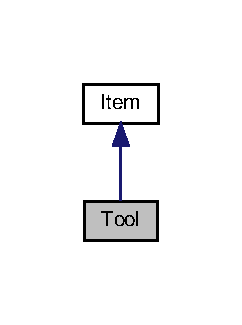
\includegraphics[width=116pt]{classTool__inherit__graph}
\end{center}
\end{figure}


Collaboration diagram for Tool\+:
\nopagebreak
\begin{figure}[H]
\begin{center}
\leavevmode
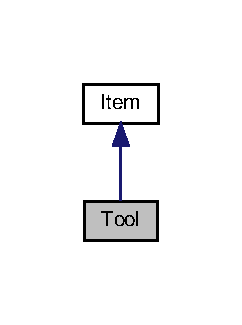
\includegraphics[width=116pt]{classTool__coll__graph}
\end{center}
\end{figure}
\subsection*{Public Member Functions}
\begin{DoxyCompactItemize}
\item 
\mbox{\Hypertarget{classTool_aa7243a0145c579be44abef01ba3bc569}\label{classTool_aa7243a0145c579be44abef01ba3bc569}} 
{\bfseries Tool} (int id, std\+::string name, int durability)
\item 
\mbox{\Hypertarget{classTool_adcd43e2f8568df819af67397ec491b94}\label{classTool_adcd43e2f8568df819af67397ec491b94}} 
\hyperlink{classTool}{Tool} \& {\bfseries operator=} (const \hyperlink{classTool}{Tool} \&other)
\item 
\mbox{\Hypertarget{classTool_afa7c7052d5eea4cdd741da20c62d0213}\label{classTool_afa7c7052d5eea4cdd741da20c62d0213}} 
int {\bfseries get\+Durability} ()
\item 
\mbox{\Hypertarget{classTool_a4d5f930a0a0993f674b5622c5362e01c}\label{classTool_a4d5f930a0a0993f674b5622c5362e01c}} 
void {\bfseries repair} (int n)
\item 
\mbox{\Hypertarget{classTool_aa979f31566ea20958ae3d01718956f2c}\label{classTool_aa979f31566ea20958ae3d01718956f2c}} 
void {\bfseries use} ()
\item 
\mbox{\Hypertarget{classTool_a3357f51a73c2e40bfea4d7f90b795b33}\label{classTool_a3357f51a73c2e40bfea4d7f90b795b33}} 
string {\bfseries output} (int qty) override
\end{DoxyCompactItemize}
\subsection*{Additional Inherited Members}


The documentation for this class was generated from the following file\+:\begin{DoxyCompactItemize}
\item 
Tool.\+hpp\end{DoxyCompactItemize}

%--- End generated contents ---

% Index
\backmatter
\newpage
\phantomsection
\clearemptydoublepage
\addcontentsline{toc}{chapter}{Index}
\printindex

\end{document}
